\documentclass{article}
\usepackage[utf8]{inputenc}
\usepackage{amsmath, amsfonts} 
\usepackage{enumitem}
\usepackage{graphicx}
\usepackage{mathtools}
\newcommand{\ddt}[1]{\frac{\partial #1}{\partial t}}
\newcommand{\dddt}[1]{\frac{\partial^2 #1}{\partial t^2}}
\newcommand{\ddx}[1]{\frac{\partial #1}{\partial x}}
\newcommand{\dddx}[1]{\frac{\partial^2 #1}{\partial x^2}}
\newcommand{\bracket}[1]{\left[ #1 \right]}
\newcommand{\paren}[1]{\left( #1 \right)}
\newcommand{\braket}[1]{\left\langle #1 \right\rangle}
\newcommand{\intinf}{\int_{-\infty}^\infty}
\newcommand{\intzinf}{\int_{0}^\infty}
\newenvironment{problem}{\begin{enumerate}[label=(\alph*)]}{\end{enumerate}}

\title{Chapter 2 Problems}
\author{William Arnold}
\date\today

\begin{document}
\maketitle 

\section*{Problem 2.1}
  Prove the following theorems:
  \begin{problem}
    \item For normalizable solutions, the separation constant $E$ must be \textit{real}

      Assume $E$ is complex, meaning $E = a + ib$ for some $a,b \in \mathbb{R}$. For a separable solution $\Psi(x, t) = \psi(x) e^{-iEt/\hbar}$, we have that
      \begin{align*}
        |\Psi(x,t)|^2 &= |\psi|^2 \left|e^{-i(a+ib)t/\hbar}\right|^2 \\
                      &= |\psi|^2 \left|e^{-iat/\hbar} e^{bt/\hbar}\right|^2 \\
                      &= |\psi|^2 e^{2bt/\hbar}
      \end{align*}
      For $t=0$, we know that $\intinf |\Psi(x,0)|^2 dx = 1$ so
      $$ \intinf |\Psi(x,0)|^2 dx = \intinf |\psi|^2 e^0 dx = \intinf |\psi|^2 dx = 1$$
      Now for any $t > 0$, we have
      $$ \intinf |\Psi(x,t)|^2 dx = \intinf |\psi|^2 e^{2bt/\hbar} dx = e^{2bt/\hbar}\intinf |\psi|^2 dx = e^{2bt/\hbar} = 1$$
      Taking the natural log of both sides we see
      $$ 2bt/\hbar = 0 $$
      and hence $b = 0$ and $E$ is composed of only the real component.

    \item The time independenent wave function $\psi$ can always be taken to be \textit{real} (unlike $\Psi$ which is necessarily complex). 
      That doesn't mean that every solution to the time-independent Schroedinger equation is real; what it says is that if you've got one that is not, it can always be expressed as a linear combination of solutions (with the same energy) that are real. So you might as well stick to $\psi$s that are real.
      
      Assume $\psi = a + ib$ is a solution to the time-independent Schroedinger equation
      $$ -\frac{\hbar^2}{2m}\dddx{\psi} + \psi V = \psi E $$
      Since both $\psi$ and $\psi^*$ solve this, we can plug both in to this equation:
      \begin{align*}
        -\frac{\hbar^2}{2m}\paren{\dddx{a} + i\dddx{b}} + (a + ib) V &= (a + ib) E \\
        -\frac{\hbar^2}{2m}\paren{\dddx{a} - i\dddx{b}} + (a - ib) V &= (a - ib) E 
      \end{align*}
      Adding these equations together we get
      \begin{align*}
        -&\frac{\hbar^2}{2m}\paren{2\dddx{a} + i\dddx{b} - i\dddx{b}} + (2a + ib - ib) V &= (a + ib - ib) E \\
        -&\frac{\hbar^2}{2m}\paren{2\dddx{a}} + 2aV = 2aE \\
        -&\frac{\hbar^2}{2m}\paren{\dddx{a}} + aV = aE
      \end{align*}
      And hence $a = \frac{1}{2} \paren{\psi + \psi^*}$ is also a solution, and has no imaginary component.
      It is worth noting that we should probably use $\frac{1}{\sqrt{2}} \paren{\psi + \psi^*}$ instead, so that we still have a normalized solution.

    \item If $V(x)$ is an even function, then $\psi$ can always be taken to be either even or odd.

      Assume we have some solution $\psi(x)$. Let $\gamma(x) = \psi(-x)$. We then have
      \begin{align*} 
        \ddx{\gamma}(x) &= -\ddx{\psi}(-x) \\
        \dddx{\gamma}(x) &= \dddx{\psi}(-x)
      \end{align*}
      If we look at $\gamma$ in the time-independent equation we get
      \begin{align*}
        -&\frac{\hbar^2}{2m}\dddx{\gamma}(x) + \gamma(x) V(x) = \gamma(x) E  \\
        -&\frac{\hbar^2}{2m}\dddx{\psi}(-x) + \psi(-x) V(x) = \psi(-x) E  \\
        -&\frac{\hbar^2}{2m}\dddx{\psi}(-x) + \psi(-x) V(-x) = \psi(-x) E 
      \end{align*}
     Where the last equation uses the evenness of $V$. 
     This equation also holds since the time independent equation holds for all $x \in \mathbb{R}$.
     Thus, $\psi(-x)$ is also a solution if $V$ is even.

     Now, since any linear combination of solutions is also a solution, we can use the even combination $\psi(x) + \psi(-x)$ or the odd combination $\psi(x) - \psi(-x)$ in order to get an even or odd solution to the equation.
  \end{problem}

\section*{Problem 2.2}
  Prove that $E$ must exceed the minimum value of $V(x)$ at some point. 

  \noindent Assume $E < V(x)$ for all $x$. Then we can solve for $\dddx{\psi}$ to see that
  $$ \dddx{\psi} = \frac{2m}{\hbar^2} \psi \paren{V(x) - E} $$

  This says that $\psi$ and $\dddx{\psi}$ always have the same sign, taking $\psi$ as a real solution.
  Assuming $\psi$ is $C^2$, if it ever takes a positive value, then it must continue to curve upwards in the positive direction and hence would grow unbounded.
  Symmetrically if $\psi$ takes on some negative value, it will grow unboundedly negative in the negative direction. 
  Hence, since $\psi \neq 0$ we have a contradiction and $E > V(x)$ for some $x$.

\section*{Problem 2.3}
Calculate $\braket{x}, \braket{x^2}, \braket{p}, \braket{p^2}, \sigma_x$, and $\sigma_p$ for the $n$-th stationary state of the infinite square well.
Check that the uncertainty principle is satisfied.
Which state comes closest to the uncertainty limit?

Recall that
$$\psi_n = \sqrt{\frac2a}\sin(\frac{n\pi}{a}x)$$
Thus we compute 
\begin{align*}
  \braket{x^2} &= \int_0^a x^2 |\psi_n|^2 dx \\
             &= \bracket{\frac{1}{12} \left(\frac{3 \left(a^2-2 \pi ^2 n^2 x^2\right) \sin \left(\frac{2 \pi  n x}{a}\right)-6 \pi  a n x \cos \left(\frac{2 \pi  n x}{a}\right)}{\pi ^3 n^3}+\frac{4 x^3}{a}\right)}_0^a \\
             &= \frac{a^2 \left(4 \pi ^3 n^3+3 \sin (2 \pi  n)-6 \pi  n (\pi  n \sin (2 \pi  n)+\cos (2 \pi  n))\right)}{12 \pi ^3 n^3} \\
             &= \frac{a^2(4\pi^3n^3 - 6 \pi n )}{12\pi^3n^3}  \\
             &= \frac{a^2}{3} - \frac{a^2}{2\pi^2n^2}\\ 
  \braket{x} &= \int_0^a x |\psi_n|^2 dx \\
             &= \bracket{\frac{a \left(-2 \pi ^2 n^2+2 \pi  n \sin (2 \pi  n)+\cos (2 \pi  n)-1\right)}{4 \pi ^2 n^2}} \\
             &= \frac{a}{2} \text{ (I used mathematica) }
\end{align*}
Thus we have 
\begin{align*}
  \sigma_x^2 &= \braket{x^2} - \braket{x}^2 \\
             &= \frac{a^2}{3} - \frac{a^2}{2\pi^2n^2} - \frac{a^2}4 \\
             &= a^2 \paren{\frac{1}{12} - \frac{1}{2n^2\pi^2}} \\
\end{align*}
It makes sense that the standard deviation would scale linearly with the area.
\begin{align*}
  \braket{p} &= \int_0^a \psi^* \bracket{-i\hbar \ddx{\psi}} dx \\
             &= \int_0^a \frac{-2\hbar i n \pi \cos(\frac{n \pi x}{a}) \sin(\frac{n\pi x}{a})}{a^2} dx \\
             &= \bracket{\frac{\hbar i \cos(\frac{2 n \pi x}{a})}{2a}}_0^a \\
             &= 0  \\
  \braket{p^2} &= \int_0^a \psi^* \bracket{-\hbar^2 \dddx{\psi}} dx \\
               &= \int_0^a \frac{1}{a^3} 2\hbar^2 n^2 \pi^2 \sin^2(\frac{n\pi x}{a}) \\
               &= \frac{\hbar^2 n^2 \pi^2}{a^2}
\end{align*}
Thus $\sigma_p^2 = \braket{p^2} = \frac{\hbar^2 n^2 \pi^2}{a^2}$

We can use this to check the uncertainty principle:
\begin{align*}
  \sigma_x \sigma_p &= \paren{\frac{\hbar n \pi}a} \paren{a \sqrt{\frac{1}{12} - \frac{1}{2n^2\pi^2}}} \\
                    &> \hbar n \pi \frac{1}{2\sqrt{3}} \\
                    &> \hbar / 2
\end{align*}
This quantity is minimized for $n = 1$

\section*{Problem 2.5}
A particle in the infinite square well has its initial wave function an even mixture of the first two stationary states:
$$\Psi(x, 0) = A[\psi_1(x) + \psi_2(x)]$$

\begin{problem}
  \item Normalize $\Psi(x, 0)$:
    \begin{align*}
      1 = \intinf |\Psi(x, 0)|^2 dx &= \intinf A^2(\psi_1^* \psi_1 + \psi_1^*\psi_2 + \psi_2^* \psi_1 + \psi_2^* \psi_2)dx \\
                                    &= A^2 \paren{\intinf |\psi_1|^2 dx + \intinf |\psi_2|^2 dx} \\
                                    &= 2A^2 \\
    \end{align*}
    Thus $A = 1/\sqrt{2}$.
  \item Find $\Psi(x,t), |\Psi(x,t)|^2$. Express the latter as a sinusoidal function of time, as in example 2.1. Let $\omega = \pi^2\hbar / 2ma^2$.
      
    We have that $c_1, c_2 = 1/\sqrt{2}$. Thus we have
    $$\Psi(x, t) = \frac{1}{\sqrt{a}}\bracket{\sin\paren{\frac{\pi x}{a}}e^{-i\omega t} + \sin\paren{\frac{2 \pi x}{a}}e^{-4i\omega t}}$$
    See the attached mathematica notebook in which we compute that
    $$|\Psi(x, t)|^2 = \frac{\sin ^2\left(\frac{\pi  x}{a}\right) \left(4 \cos \left(\frac{\pi  x}{a}\right) \cos (3 t \omega)+2 \cos \left(\frac{2 \pi  x}{a}\right)+3\right)}{a}$$

  \item Compute $\braket{x}$. Notice that it oscillates in time. What is the angular frequency of the oscillation? What is the amplitude of the oscillation?
    
    Using mathematica we see that
    $$ \braket{x} = \frac{a}{2}-\frac{16 a \cos (3 t\omega)}{9 \pi ^2}$$
    
    The amplitude of this oscillation is $16a/9\pi^2$ and it's frequency is $3\omega$.

  \item Compute $\braket{p}$.

    Here we can use that $\braket{p} = m \frac{d}{dt}\braket{x}$:

    \begin{align*}
      \braket{p} &= m \frac{16a\omega}{3\pi^2} \sin(3t\omega) \\
                 &= \frac{8\hbar}{3a} \sin(3t\omega)
    \end{align*}

  \item If you measured the energy of this particle, what possible values could it's energy be and with what probabilities? Find the expectation value of $H$. How does it compare with $E_1, E_2$.

    The two possible values we could get are $E_1 = \omega, E_2 = 4 \omega$. 
    Since $c_1, c_2 = 1/\sqrt{2}$, we get either $E_1$ or $E_2$ with probability $1/2$.

    \begin{align*}
      \braket{H} &= \intinf \Psi^* \hat{H} \Psi dx \\
                 &= \intinf \Psi^* \frac{1}{\sqrt{2}}\paren{E_1 \psi_1 + E_2 \psi_2} dx \\
                 &= \frac{1}{2} \intinf \bracket{E_1 \psi_1^* \psi_1 + E_1 \psi_2^* \psi_1 + E_2 \psi_1^* \psi_2 + E_2 \psi_2^* \psi_2}dx \\
                 &= \frac{1}{2} \paren{E_1\intinf \psi_1^* \psi_1 dx + E_2 \intinf \psi_2^* \psi_2 dx} \\
                 &= \frac{E_1 + E_2}{2}
    \end{align*}

    Which, as we would expect is $\braket{E}$.

\end{problem}

\section*{Problem 2.7}

A particle in the infinite square well has the initial wave function 
$$\Psi(x, 0) = \begin{cases}
  Ax & 0 \leq x \leq a/2 \\
  A(a-x) & a/2 \leq x \leq a 
\end{cases}$$

\begin{problem}
\item Sketch $\Psi(x, 0)$ and determine $A$.

  \centerline{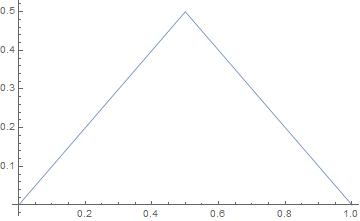
\includegraphics[width=2in]{2-7a.jpg}}

  \begin{align*}
    \intinf |\Psi(x, 0)|^2 &= A^2\int_0^{a/2} x^2 dx + A^2 \int_{a/2}^a (a-x)^2 dx \\ 
                           &= A^2 \paren{\bracket{x^3/3}_0^{a/2} + \bracket{-(a-x)^3/3}_{a/2}^a}A \\
                           &= A^2 \paren{\frac{a^3}{24} + \frac{a^3}{24}} \\
                           &= \frac{A^2 a^3}{12} = 1
  \end{align*}
  Thus $A = \sqrt{12/a^3}$

\item Find $\Psi(x, t)$.

  This amounts to determining the $c_n$.
  Using mathematica we see that 
  $$c_n = \frac{4 \sqrt{6} \sin \left(\frac{\pi  n}{2}\right)}{\pi ^2 n^2}$$
  Thus we have 
  $$ \Psi(x, t) = \sum_{n=0}^\infty \frac{4 \sqrt{6} \sin \left(\frac{\pi  n}{2}\right)}{\pi ^2 n^2} \sqrt{\frac{2}{a}} \sin\paren{\frac{n \pi}{a} x} e^{-i t n^2 \pi^2 \hbar / 2 m a^2} $$

\item What is the probability we measure the energy $E_1$?

  This is $$|c_1|^2 = \frac{96}{\pi^4}$$

\item Find the expectation value of the energy:

  \begin{align*}
    \braket{H} &= \sum_{n=1}^\infty |c_n|^2 E_n = \sum_{n=1}^\infty \frac{96 \sin^2 \left(\frac{\pi  n}{2}\right)}{\pi ^4 n^4} \frac{n^2 \pi^2 \hbar^2}{2 m a^2} \\
               &= \frac{48 \hbar^2}{\pi^2 ma^2} \sum_{n=1}^\infty \frac{\sin^2(\pi n / 2)}{n^2} \\
               &= \frac{48 \hbar^2}{\pi^2 ma^2} \paren{1 - \frac1{3^2} + \frac1{5^2} - \frac1{7^2} + ..} \\
               &= \frac{48 \hbar^2}{\pi^2 ma^2} \frac{\pi^2}{8} \\
               &= \frac{6 \hbar^2}{ma^2}
  \end{align*}

\end{problem}



\section*{Problem 2.10}

  \begin{problem}
    \item Construct $\psi_2(x)$
      
      Using mathematica we get that 
      $$ \psi_2(x) = \frac{\sqrt[4]{m \omega } e^{-\frac{m x^2 \omega }{2 \hbar }} \left(2 m x^2 \omega -\hbar \right)}{\sqrt{2} \sqrt[4]{\pi } \hbar ^{5/4}} $$

    \item Sketch $\psi_0, \psi_1, \psi_2$:

      \centerline{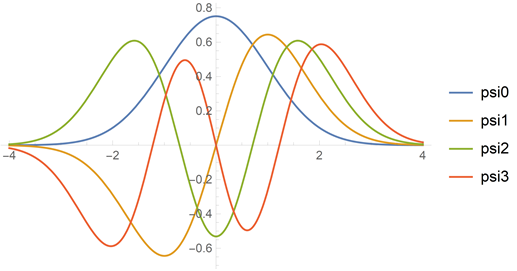
\includegraphics[height=2.5in]{2-10b-psis.png}}

    \item Check orthogonality (see mathematica)
  \end{problem}

\section*{Problem 2.11}

  \begin{problem}
    \item Compute $\braket{x}, \braket{p}, \braket{x^2}, \braket{p^2}$ for $\psi_0, \psi_1$


  \end{problem}
\end{document}

